%% Geometry of circles %%
% Question 4
\hlquestion Find the points of intersection of the line 
$y = 2x + 1$ 
and the circle 
$x^{2} + y^{2} - 2y - 4 = 0$.
Show that the line 
$y = 2x + 1$ 
is a diameter of the circle. 
Find the equation of the tangent to the circle at one of the points of 
intersection.

\begin{solution}
	BE note: $(1 - r^{2} = -4) \rightarrow r^{2} = 5$
	\[
		(x+0)^{2} + (y-1)^{2} = 5
	\]
	\[
		\therefore
		\text{centre} \; 
		(0, 1)
		,\; \text{radius} = 
		\sqrt{5}
	\]
	\underline{Part 1: find points of intersection}
	\par
	Sub $(y=2x+1)$ into $(x^{2} + y^{2} - 2y + 4 = 0)$
	\[
		\rightarrow
		x^{2} + (2x+1)^{2} - 2(2x+1) + 4 = 0
	\]
	\[
		x^{2} + 4x^{2} + 4x - 4x + 1 - 2 - 4 = 0
	\]
	\[
		5x^{2} = 5
	\]
	\[
		x = \pm 1
	\]
	Sub into: 
	\[
		y=2x+1	
	\]
	\begin{multicols}{2}
		Intersection 1: when $x=1$,
		\[
			y = 2+1 
			\; 
			(= 3)
		\]
		\[
			\underline{
				(1, 3)
			}
		\]		
		Intersection 2: when $x=-1$,
		\[
			y = -2+1 
			\; 
			(= -1)
		\]
		\[
			\underline{
				(-1, -1)
			}
		\]
	\end{multicols}
	\underline{Part 2: show that the line is a diameter of the circle}
	\par
	Midpoint of two points is $(0, 1)$ which is also the centre of the circle
	\[
		\underline{
			\therefore
			y=2x+1 
			\; 
			\text{is a diameter of the circle}
		}
	\]
	\underline{Part 3: calculate tangent at each point}
	\[
		m_{1} = 2 
	\]
	\[
		\rightarrow
		m_{2} = -\frac{1}{2}
	\]
	\begin{multicols}{2}
		$\therefore$ at (1, 3)
		\newline
		Using $y=mx+c$ to find $c$
		\[
			\rightarrow
			(3) = -\frac{1}{2} (1) + c
		\]
		\[
			c = \frac{7}{2}
		\]	
		\qSolMath{
			\therefore
			y = -\frac{1}{2} x + \frac{7}{2}
		}{}
		\[
			\text{or}
			\;\; 
			2y + x = 7
		\]
		$\therefore$ at (-1, -1)
		\newline
		Using $y=mx+c$ to find $c$
		\[
			\rightarrow
			(-1) = -\frac{1}{2} (-1) + c
		\]
		\[
			c = -\frac{3}{2}
		\]	
		\qSolMath{
			\therefore
			y = -\frac{1}{2} x - \frac{3}{2}
		}{}
		\[
			\text{or}
			\;\; 
			2y + x = -3
		\]
	\end{multicols}
	\underline{Diagram:}
	\begin{center}
		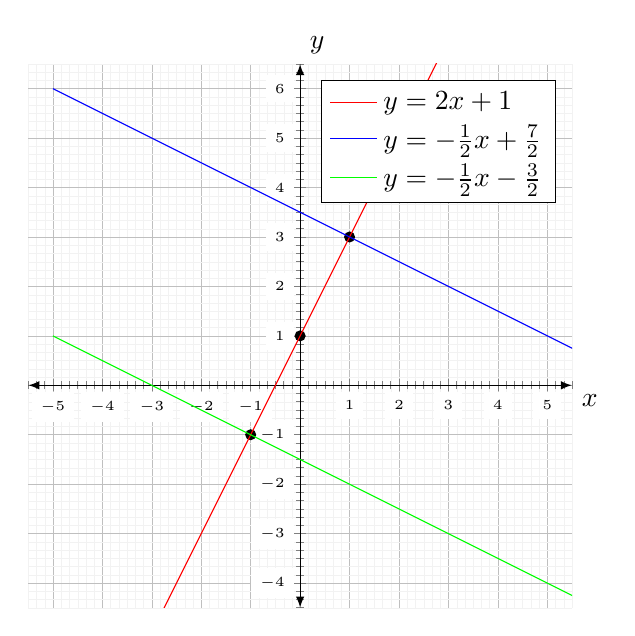
\begin{tikzpicture}
			\begin{axis}[
					width=0.7\textwidth,
					height=0.7\textwidth,
					xtick distance=1,
					ytick distance=1,
					xmin=-5.0,xmax=5,
					ymin=-4.0,ymax=6,
					xlabel = $x$,
					ylabel = $y$,
					grid=both,
					grid style={line width=.1pt, draw=gray!10},
					major grid style={line width=.2pt,draw=gray!50},
					axis lines=middle,
					minor tick num=5,
					enlargelimits={abs=0.5},
					axis line style={latex-latex},
					ticklabel style={font=\tiny,fill=white},
					xlabel style={at={(ticklabel* cs:1)},anchor=north west},
					ylabel style={at={(ticklabel* cs:1)},anchor=south west},
					legend pos=north east,
					legend entries={
						$y = 2x + 1$,
						$y = -\frac{1}{2} x + \frac{7}{2}$,
						$y = -\frac{1}{2} x - \frac{3}{2}$,
					},
					legend cell align={left},
				]
				\fill (axis cs: 0, 1) circle[radius=2pt];
				\draw (axis cs: 0, 1) circle[radius=22.36]; %sqrt(5)=2.23606798
				
				\fill (axis cs: 1,   3) circle[radius=2pt];
				\fill (axis cs: -1, -1) circle[radius=2pt];

				\addplot[
					domain=-5:11, 
					samples=100, 
					color=red,
				]
				{ (2*x) + 1};
				\addplot[
					domain=-5:11, 
					samples=100, 
					color=blue,
				]
				{ -(1/2)*x + (7/2)};
				\addplot[
					domain=-5:11, 
					samples=100, 
					color=green,
				]
				{ -(1/2)*x - (3/2)};
			\end{axis}
		\end{tikzpicture}
	\end{center}
		
\end{solution}

\appenddata{questionSolutions}{
{
	The points of intersection are $(1, 3)$ and $(-1, -1)$. 
	The mid-point of these is $(0, 1)$ which is
	the centre of the circle, and hence $y = 2x + 1$ is a diameter. 
	The tangents are 
	$2y + x = 7$ 
	and
	\hl{$2y + x = -3$}
	respectively.
}
}